\chapter{Vergleich und Auswahl}
% ehemals Lösungsweg

In diesen Kapitel wird erörtert, welche Technologie (Xtext oder Scala) für
dieses Projekt am praktikabelsten ist und sich somit schlussendlich durchsetzt.
Kern hierfür ist die Übersicht in Form einer Vergleichsmatrix in Abschnitt
\ref{sec-vergleichsmatrix}.

\section{Warum Scala bzw. Xtext?}\label{sec-warumAusgewaehlt}

\paragraph{Scala}
hat ausgezeichnete Fähigkeiten zur Gestaltung einer
internen DSL, nähere Details siehe Kapitel \ref{sec-grammatikGestaltung},
und als objekt-orientierte sowohl auch funktionale Sprache sehr
vielfältige Möglichkeiten für den Benutzer bietet, egal ob er sich
gerade „innerhalb“ der DSL gefindet oder „standard“ Scala schreiben
möchte. Zudem hat Scala eine sehr aktive Community und wird vom
Universitätzlehrstuhl unter Martin Odersky weiterentwickelt.
Zudem ist Scala ein OpenSource-Projekt.
Durch die Fähigkeit auf der Java Virtual Machine (JVM) zu laufen,
hat Scala auch eine sehr gute Integration mit Java und
Java-Bibliotheken.

\paragraph{Xtext} ist ein Framework welches auf die Entwicklung externer DSLs
ausgelegt ist und dabei auf die Eclipse IDE Plattform aufbaut
und sehr viel der harten Arbeit abnimmt, was die Entwicklung
externer DSLs nachhaltig vereinfacht.
Auch Xtext läuft auf der JVM und ist stark mit Java integriert, bringt
zudem eine eigene, auch mit Xtext entwickelte, Sprache mit. Diese von der
Syntax her freundlicher als Java ist, aber sich dennoch nahe an den
Java-Konzepten aufhält. Diese Sprache heißt Xtend und wird vornehmlich
intern zur Generator-Programmierung eingesetzt.
Auch Xtext ist ein OpenSource-Projekt und wird hauptsächlich von der
deutschen Firma \emph{itemis AG} betreut bzw. weiterentwickelt.

Ein genauerer Vergleich
zwischen Scala und Xtext findet sich in Kapitel \ref{sec-vergleichsmatrix}.

\section{Vergleichsmatrix}\label{sec-vergleichsmatrix}

In dieser Tabelle ist eine Übersicht über den Vergleich gegeben, indem
die Fähigkeiten bzw. die Möglichkeiten von Xtext als externe DSL und
Scala als interne DSL gegenübergestellt werden.

Für \emph{einige} der gelisteten Fähigkeiten gibt es
tiefergehende Beschreibungen, auf diese
in der ersten Spalte der Tabelle entsprechend referenziert wird.

\begin{landscape}
\begin{longtable}{|p{0.5cm}|p{0.8cm}|p{4.3cm}|p{6.3cm}|p{6.3cm}|}

  \hline
  Nr. & Kap. & Fähigkeit & Xtext (externe DSL) & Scala (interne DSL) \\ \hline \hline
  \endfirsthead

  \hline
  Nr. & Kap. & Fähigkeit & Xtext (externe DSL) & Scala (interne DSL) \\ \hline
  \endhead

  1
  & \ref{sec-grammatikGestaltung}
  & Grammatikalische Gestaltung der DSL
  & Komplett frei und flexibel, da in BNF-Regeln definiert.
  & Eingeschränkt, man bleibt an Scala's Beschränkungen gebunden, aber
    dennoch sehr ausdrucksstarke Möglichkeiten.
  \\\hline

  2
  & \ref{sec-gpl}
  & DSL mit General Purpose mischbar
  & Hat viele Hürden, um eine DSL mehr Allgemeingültigkeit zu verpassen.
  & Alle Scala-Fähigkeiten nativ nutzbar, da die DSL eine normale Library ist.
  \\\hline

  3
  & \ref{sec-strukturierungsfaehigkeit}
  & Strukturierungsfähigkeit des Codes
  & Muss alles selbst gebaut werden. Vorteil: Es muss nur das nötigste
    umgesetzt werden.
  & Sämtliche Infrastruktur vorhanden. (Packages, Kontrollstrukturen,
    Build-Tools, ...)
  \\\hline

  4
  & \ref{sec-erweiterbar}
  & Erweiterbarkeit durch Domain User/Community (z.B. für eigene Templates)
  & Es würde von dem Domain User verlangt werden BNF-Notation zu können,
    Xtend und er wäre auf Eclipse gezwungen. % da kann sich fast gar keine Community bilden
  & Einfache Scala Kenntnisse plus eine kleine Anleitung sollten ausreichen,
    die Bindings zu erstellen.
  \\\hline

  5
  & \ref{sec-erweiterbar}
  & Erweiterbarkeit durch Entwickler
  & Grammatik, Tests und Generator kann nach belieben wachsen, u.a.
    Unterstützung durch Eclipse.
  & Der Aufwand liegt bei der Entwicklung einer Library. Jedoch müssen
    Testumgebungen etc. selbst eingerichtet werden.
  \\\hline

  6
  & \ref{sec-erweiterbar}
  & Wiederverwendbarkeit bzw. Kombination mit Vorhandenem
  & Nur eingeschränkt, jedoch sind Grammatik Mixins möglich.
  & Sehr gut, da Library und mit Scalas Typ- und Vererbungssystem kann nach
    gewohnter Manier kombiniert und erweitert werden.
  \\\hline

  7
  & \ref{sec-infrastruktur}
  & Sprach-Infrastruktur
  & Xtext generiert automatisch ein speziell angepasstes Eclipse Plugin.
  & Alles wird mitgeliefert, wie z.B. Compiler, Built-Tools, REPL.
    Breite Unterstützung von vielen Editoren.
  \\\hline

  8
  & \ref{sec-scalierEinbett}
  & Einbettbarkeit in beliebige Umgebungen
  & De facto Eclipse-Bindung, aber mit individuell angepasstem Eclipse-Plugin,
    welches sich mit dem Projektverlauf automatisch mit anpassen kann.
    Wenn das Ziel ein Arbeitsplatz-Front-End ist, sehr vorteilhaft -- sofern
    Eclipse eingesetzt werden will.
  & Kann gut in alle möglichen Szenarien eingebettet werden, Benutzung
    innerhalb eines Frameworks möglich, oder einsatz als Bibliothek,
    Stand-Alone oder in einer Entwicklungsumgebung wie Eclipse denkbar.
    Kann also quasi in eine beliebige Umgebung eingebettet werden
    wo eine JVM läuft oder auch als Service bereitgestellt werden.
    Allerdings ist Xtext in Eclipse besser eingebunden, da speziell angepasst.
  \\\hline

  9
  & \ref{sec-generator}
  & Generator: Zielplatform
  & Ohne Umwege kann jede Sprache oder Markup aus dem DSL-Modell durch eine
    Template-Engine generiert werden, das Eclipse-Plugin stellt sofort das
    Generat bereit. Jedoch kann nativer Code nicht direkt auf Xtext laufen,
    es muss also ggf. noch ein externer Build o.ä. angestossen werden.
  & Die DSL selbst kann direkt ein lauffähigkes Programm sein. Andere Ziele,
    z.B. andere Programmier-Sprachen oder Markup-Sprachen müssen einen Umweg
    über eine Template-Engine nehmen, allerdings steht hier ein Eclipse-Plugin
    bereit, welches direkt nach jeder Änderung das Generat bereitstellt; das
    Verfahren hierzu muss selbst entwickelt werden (das kann ein Vor- oder
    auch ein Nachteil sein.)
  \\\hline

  10
  & \ref{sec-generator}
  & Generator: Template-Engine
  & Xtend eine speziell angepasste DSL-Generator-Template-Engine.
    Die BNF-Grammatik wird transparent in Java- bzw. Xtend-Klassen übersetzt,
    mit denen das Ziel über das Template generiert werden kann.
  & 1. Freie Wahl, z.B. einface Multiline-Strings, Scala XML oder Scalate;
    wie aus der internen DSL das Ziel generiert wird, benötigt in der Regel
    einen Zwischenschritt (Bindings), welcher programmiert werden muss.
    Scala kann jedoch ggf. das Generat als Unterprogramm ausführen.
    2. Die interne DSL ist selbst lauffähig.
  \\\hline

  11
  &
  & Entwicklungsaufwand (u.a. Zeit, Einarbeitung)
  & Wenn BNF-Kenntnisse (theoretische Informatik) vorhanden sind,
    relativ leichte Einarbeitung.
    Die Tools nehmen die harte Arbeit ab. Es gibt schon standardisierte
    Vorgehensweisen, z.B. wie der Generator gebaut wird.
  & Wenn Scala-Kenntnisse vorhanden, ist es mehr oder weniger die Entwicklung
    einer Bibliothek.
    Wie man den Generator baut, muss allerdings überlegt werden.
  \\\hline

  12
  & \ref{sec-erweiterbar}
  & Software-Lebenszyklus und Wartbarkeit
  & Dank IDE und einer schon eingerichteten Testumgebung, also sehr gut.
  & Man hat alle Möglichkeiten, die die Scala-Welt bietet, also sehr gut.
    Jedoch ist Handarbeit nötig.
  \\\hline

  13
  &
  & Tooling (für DSL Gestaltung)
  & Komplette und entsprechend angepasste Eclipse Entwicklungsumgebung.
  & Die Sprache selbst, sonst keine Hilfen.
  \\\hline

  14
  & \ref{sec-scalierEinbett}
  & Skalierbarkeit
  & Kommt auf das Generat an. Man ist und bleibt an Eclipse gebunden.
  & Scala selbst ist in alle Richtungen (Größe, Nebenläufigkeit) sehr gut
    skalierbar.
  \\\hline

  15
  &
  & DSL als Library bzw. Bereitstellung
  & Ist eine in sich mehr oder weniger geschlossene Struktur.
  & Interne DSL ist eine ganz normale Scala Library.
  \\\hline

\end{longtable}
\newpage
\end{landscape}


\subsection{Sprach-Infrastruktur}\label{sec-infrastruktur}

\paragraph{Xtext} wird direkt als fertig eingerichtete Eclipse IDE
ausgeliefert, die speziell an die Erstellung von externen DSLs angepasst
ist. Es wird also ein DSL-Erstellungs-Ökosystem „out-of-the-box“ geliefert.

Xtext bietet die folgenden Dinge, mit einer exzellenten IDE Unterstützung:

\begin{itemize}
  \item Grammatik DSL (BNF-ähnlich),
  \item unterschiedliche Code-Generatoren (siehe. Abschnitt \ref{sec-generator}),
  \item an DSL-Entwicklung angepasste Testumgebung (z.B. Unittests.)
\end{itemize}

Zudem sei erwähnt, dass Xtext aus den Grammatik-Regeln automatisch ein
passendes Eclipse-Plugin generiert, welches die Grammatik vollständig
unterstützt, wie z.B. Syntax-Hervorhebung, Überprüfung der grammatikalischen
Korrektheit oder Auto-Vervollständigung.

Weiter werden aus den Grammatik-Regeln Java-Klassen abgeleitet, mit denen
komfortabel die Code-Generierung vorgenommen werden kann. Der DSL-Programmierer
muss sich also nicht mit abstrakten Syntaxbäumen oder Ähnlichem herumschlagen.

\paragraph{Scala} bringt als vollwertige \emph{General Purpose Language}
ein umfangreiches Ökosystem mit, bestehend aus verschiedenen Werkzeugen
und vielen Bibliotheken, beispielsweise eine mächtige Standard-Bibliothek.
Hervorzuheben sind:

\begin{itemize}
  \item Linker und Compiler,
  \item Built-Tools wie \emph{sbt} mit Abhängigkeits-Management,
  \item Read-Evaluate-Print-Loop (REPL), eine interaktive Scala-Sitzung,
  \item Zugriff auf die Java-Standard-Library,
  \item Umfangreiche Scala-Standard-Library.
\end{itemize}

Darüber hinaus hat Scala sehr gute Fähigkeiten zur Erstellung von internen
DSLs, siehe Abschnitt \ref{sec-grammatikGestaltung}.


\subsection{Strukturierungsfähigkeit}\label{sec-strukturierungsfaehigkeit}

Im Allgemeinen ist mit der Strukturierungsfähigkeit gemeint, wie der
geschriebene (DSL-)Code logisch und sinnvoll gegliedert werden kann,
z.B. durch

\begin{itemize}
  \item Pakete, Module oder Namensräume,
  \item Klassen oder Objekte,
  \item Funktionen bzw. Geltungsbereiche,
  \item eventuell auch Kontrollstrukturen oder Datenstrukturen.
\end{itemize}

Fehlerbehandlung ist auch ein wichtiger Posten, also ob Ausnahmen
geworfen werden können. Hier hat Xtext Eclipse als Helfer, der
z.B. Syntax-Fehler ausfindig machen kann und Scala hat u.a. den Compiler
und Ausnahmen die zur Laufzeit geworfen werden können.

\paragraph{Xtext} ermöglicht es von Grund auf eine Sprache zu entwickeln,
die komplett auf das Domänen-Problem zugeschnitten ist -- ohne Kompromisse.
Dadurch dass die Sprache von Grund auf erstellt wird, ist der Entwickler
auch dazu gezwungen sich Gedanken dazu zu machen, wie der DSL-Code
der vom Domain-Benutzer geschrieben wird strukturiert werden kann,
was insbesondere bei größeren DSL-Skripten oder
Projekten günstig sein kann -- falls gewünscht bzw. gebraucht.
Jedoch ist Handarbeit erfolderlich, um solche Fähigkeiten wie sie o.g.
sind in der DSL unter zu bekommen.

\paragraph{Scala} bietet die o.g. Struktuierungsfähigkeiten generisch an,
es muss also keinerlei Aufwand getrieben werden, um die interne DSL mit
diesen Fähigkeiten auzustatten. Soll heißen, all das wird gratis mitgeliefert.


\subsection{General Purpose Language}\label{sec-gpl}

Im Gegensatz zu DSLs stehen \emph{General Purpose Languages}, kurz GPLs.
Das soll heißen, dass mit diesen Sprachen alle Probleme gelöst werden, da
sie turing-vollständig sind.

Hauptunterschiede zwischen DSLs und GPLs sind,

\begin{itemize}
  \item eine DSL zielt auf ein spezifisches Problemfeld ab,
  \item eine DSL enthält Syntax und Semantik, welches sich auf dem gleichen
        Abstraktionslevel wie das der Domäne befindet.
\end{itemize}

(\cite{dsls}, Seite 11)

Das bedeutet, dass das DSL-Skript die unterliegende Implementierung abstrahieren
muss. Es düfen also möglichst keine Implementierungsdetails darin auftauchen.
(\cite{dsls}, Seite 15)

Jetzt kann es sein dass, wie in diesem Projekt gewünscht,
auch die Möglichkeit geboten wird universellen Programmcode zu schreiben,
um z.B. auf das Dateisystem zuzugreifen oder eine Grafik mit einer
externen Bibliothek zu erstellen. Der Domain-Benutzer soll also die
Möglichkeit haben, die DSL zeitweise zu verlassen um „normalen“ Programmcode
zu schreiben und danach wieder in die DSL zurückzukehren---ohne große
Aufwand.

Dies ist für dieses Projekt relativ wichtig, dass auch GPL-Elemente zugelassen
werden, um eine möglichst hohe Automatisierung der Dokumentenerstellung
dem Benutzer zu ermöglichen. Siehe dazu als Beispiele
die verschiedenen Szenarien aus Kapitel \ref{sec-idee-szenarien}.

\paragraph{Xtext} bietet die Möglichkeit mittels Xbase GPL-Expressions
auszuführen -- und das obwohl Xtext externe DSLs erstellt, für die es für
gewöhnlich eine sehr harte Arbeit darstellt GPL-Elemente einfließen zu lassen.
Xtext vereinfacht diese harte Arbeit. Aber auch hier ist die Implementierung
nicht ganz kostenfrei, da als Generator nur noch der \emph{ModelInferrer}
(siehe Abschnitt \ref{sec-generator}) zum Einsatz kommen kann.
Und auch hier hat man nicht die absolute Freiheit, die man sich eventuell
wünschen würde:

\begin{itemize}
  \item Falls sich der Geltungsbereich von DSL und GPL-Abschnitt überschneiden
        soll, kann es zu Komplikationen kommen, z.B. wenn der DSL-Code
        auf eine Variable aus dem GPL-Abschnitt zugreifen soll (siehe
        Abschnitt \ref{sec-forwardreference}.)
  \item Der ModelInferrer kann nur noch Java bzw. die JVM als Ziel haben.
\end{itemize}

\paragraph{Scala} ist eine GPL und hier in dem Projekt wird eine interne
DSL mit Scala erstellt. Dort gibt es absolut keine Einschränkungen, es
kann auf den vollen Funktionsumfang von Scala zugegriffen werden.
Da die interne DSL quasi nur eine ausdrucksstarke Scala-Bibliothek ist,
können die Grenzen der DSL mit der GPL verschwimmen.


\subsection{Erweiterbarkeit, Wiederverwendbarkeit und Wartbarkeit}
\label{sec-erweiterbar}

In diesem Projekt ist es sehr wichtig, dass sowohl DSL als auch
die Geschäftslogik flexibel erweiterbar sein soll bzw. sogar
einzelne Teile wiederverwenden zu können.

Warum ist das so wichtig? Weil im späteren Lebenszyklus dieser Software
verschiedenartige Dokumente generierbar sein sollen, wo im Idealfall
die Domain-Benutzer selber Änderungen an den Bindungen zwischen
Dokumenten-Template und der DSL vornehmen können. Die Domain-Benutzer
wollen eventuell das Dokument um neue Arten von Darstellungen (z.B. spezielle
Tabellen) oder gänzlich neue Möglichkeiten (z.B. ein Chemie-Editor
innerhalb des resultierenden Dokuments) erweitern.
Verschiedene Dokumenten-Arten sollen sich leicht hinzufügen lassen,
z.B. zum einen ein akademischer Bericht, zum anderen ein europäisches Patent.

Eventuell möchte man auch Bestandteile aus z.B. dem Patent-Template in
einem anderen Template wiederverwenden? Das Ziel ist also eine
möglichst lebendige Umgebung, mit der Fähigkeit leicht erweiterbar zu sein.

\paragraph{Xtext} hat hier den Hauptnachteil, dadurch dass quasi nur
Entwickler in der Lage sind die Grammatik zu erweitern oder den
Generator zu pflegen. Aber die Domain-Benutzer sollen in der Lage sein
eigene Dokumenten-Templates zu erstellen oder vorhandene zu modifizieren.

\paragraph{Scala} kann hier glänzen dadurch, dass zu jedem Template auch
direkt ein Bindungs-Code vom (versierten) Domänen-Benutzer erstellt
werden kann, da die Komplexitäten in tiefere Schichten gezogen werden können.
Durch das starke Vererbungssystem welches Scala bietet, können solche
Template-Erweiterungen ohne viel unschöne Details erstellt werden, da sich
auf das Wesentliche konzentriert werden kann.


\subsection{Grammatikalische Gestaltung}\label{sec-grammatikGestaltung}

Die grammatikalische Gestaltung ist eine der wichtigsten Eingenschaften
für die Ausdrucksstärke einer DSL und die Ausdrucksstärke ist eines
der wichtigsten Kriteren für die Akzeptanz der Domain-Benutzer.

\paragraph{Xtext} ist ein Framework zur Erstellung von externen DSLs und
hat somit naturgemäß ausgezeichnete Fähigkeiten zur Gestaltung einer beliebigen
Grammatik.

Dabei setzt Xtext auf eine selbst entwickelte externe DSL, die sehr große
Ähnlichkeit mit der \emph{Backus-Naur-Form} hat, mit der kontextfreie
Grammatiken bzw. Programmiersprachen entworfen werden können.

\paragraph{Xtext Grammatik-Beispiele}

Hier zwei implementierte Beispiel-Grammatiken, um die Flexibilität von
Xtext zu verdeutlichen, einmal eine Grammatik die Ähnlichkeit mit \TeX~
hat und zum anderen eine Grammatik die an die interne DSL von Scala angelent,
jedoch entspricht diese nicht ganz dem Endresultat der Scala-DSL, ist.

\begin{lstlisting}[caption=\TeX-ähnliches Xtext-Grammatik-Snippet.]
grammar de.htwg.scaltex.latexdsl.LaTeXDSL
  with org.eclipse.xtext.common.Terminals

generate laTeXDSL "http://www.htwg.de/scaltex/latexdsl/LaTeXDSL"

Model:
  entities += Entity*;

Entity:
  Section | Paragraph;

Section:
  '\\section' '{' content = TEXT '}';

Paragraph:
  content = TEXT;

terminal TEXT  : 
  ( '\\'('b'|'t'|'n'|'f'|'r'|'u'|'"'|"'"|'\\') |
    !('\\'|'{'|'}'|'\n') )*;
\end{lstlisting}

\begin{lstlisting}[label=xtext-gramm,caption=An Scala-DSL angelente Xtext-Grammatik.]
grammar de.htwg.scaltex.dsl.ScalTeX with org.eclipse.xtext.common.Terminals

generate scalTeX "http://www.htwg.de/scaltex/dsl/ScalTeX"

Scaltex:
  'filename' name = ID
  entities += Entity*;

Entity:
  Heading | UniversalEntity | UniversalEntityWithKwargs | ControlCommand;

Heading:
  '§' order = ('>' | '>>' | '>>>') content += STRING;

UniversalEntity:
  '^' name = ID
    content = STRING;

UniversalEntityWithKwargs:
  '^' name = ID
    content = Kwargs;

ControlCommand:
  '!!' content = ID;

Kwargs:
  '('
    (arguments += Argument)*
  ')';

Argument:
  name = ID '=' content = STRING (comma = ',')?;
\end{lstlisting}

\paragraph{Scala} hat für eine Programmiersprache von sich aus schon
sehr gute Fähigkeiten zur Erstellung von internen DSLs, dies
manifestiert sich in folgenden Fähigkeiten (siehe \cite{dsls} Kapitel 6.1):

\begin{itemize}
  \item Unicode-Zeichen in Identifiern erlaubt,
  \item Methoden können als Prefix, Infix oder Postfix Operatoren dienen,
  \item flexible Syntax (z.B. optimale Punkte zum Methodenaufruf),
  \item viel syntaktischer Zucker u.a. mit impliziten Erweiterungen,
  \item Stärken von objektorientierter- und funktionaler-Programmierung
        geschickt vereint,
  \item starke statische Typesierung, jedoch ergänzt der Compiler selbstständig
        sehr viele Typ-Informationen → wirkt fast wie eine dynamisch
        typesierte Sprache.
\end{itemize}

Zudem sei erwähnt, dass es für Scala auch eine Bibliothek gibt mit
der es möglich ist externe DSLs zu entwerfen. Diese basiert der
\emph{parser combinator} Technik (siehe \cite{dsls} Kapitel 8.)

\begin{lstlisting}[caption=Scala DSL Syntax (Snippet).]
class EntityBinding {
  // ...
  def § (heading: String) = println(heading)  // new EntityHeading ...
  def txt (text: String) = println(text)  // new EntityText ...
}

class Areal {
  // ...
  val ++ : EntityBinding = new EntityBinding
  // ...
}

// Run Code

object O extends Areal {
  ++ § "My Heading"
  ++ txt "Lorem ipsum ..."
}
\end{lstlisting}

Das Objekt O erbt von Areal die Syntax. Bedeutung der Syntax ist
„plus Überschrift Entität, plus Text Entität”. Der Nachteil dabei ist,
dass leider ein + nicht allein für sich stehen kann, da der Compiler dies
als Unäre-Operation zählt und somit nicht wie gewünscht erkennt, ++ jedoch
zählt als Infix-Operation und funktioniert daher wie gewünscht.

\subsection{Skalierbarkeit und Einbettbarkeit}\label{sec-scalierEinbett}

\paragraph{Xtext} hat eine vollständige und absolute Abhängigkeit
zur Eclipse IDE und kann folglich nicht ohne Eclipse auskommen bzw.
funktionieren. Daher ist man in Sachen Skalierbarkeit bzw. Einbettbarkeit
an die Einschränkungen bzw. auch Vorteile von Eclipse gebunden.

Eclipse ist eine mächtige IDE, die auf mittlere bis große Softwareprojekte
ausgelegt ist, und somit eher unter die schwergewichtigen Entwickler-Werkzeuge
einzuordnen ist. Aber der Vorteil ist, dass selbst riesengroße Projekte
damit verwaltbar sind und das Projekt quasi nach belieben wachsen kann und
durch die Refactoring-Fähigkeiten auch leicht wartbar und erweiterbat ist.
Man könnte also sagen, dass Xtext die Skalierbarkeit von Eclipse erbt.

Das Generat kann je nach eingesetzen Generator (siehe Abschnitt
\ref{sec-generator}) skalieren, da Xtext quasi beliebige Generate erstellen
kann, muss für Einzelfall entschieden werden.

Zur Einbettbarkeit in beliebige Umgebungen, ist der Entwickler bzw.
Domain-Benutzer sehr gebunden und abhängig. Eclipse läuft für gewöhnlich
nur auf Desktop-Computern, also mit grafischer Benutzeröberfläche,
und benötigt relativ vielen Ressourcen, die Eclipse auch
gerne annimmt.
Da Eclipse auch die Generatoren anwirft, um aus der DSL
die Zielarchitektur zu erstellen, ist auch dieser Prozess an Eclipse gebunden.
Daher ist der Einsatz auf z.B. einem dedizierten Server ohne grafische
Benutzeroberfläche nicht so leicht umzusetzen.

Die Einbettbarkeit des Generats ist wieder von seinen eigenen Fähigkeiten
abhängig, also u.U. sehr gut.

\paragraph{Scala} trägt die Skalierbarkeit schon im Namen. Als
„scalable language“ und hat Scala entsprechende Fähigkeiten in alle Richtungen
zu skalieren. Beispiele: Es ist möglich Scala-Programme vom kleinen
Shell-ähnlichen Skript mit 2 Zeilen, bis hin zur Enterprise Software
mit hunderttausenden Zeilen Code zu schreiben. Also vom kleinen mini
Einzelplatzskript bis zu Mainfraimapplikationen mit unzähligen nebenläuftigen
Zugriffen.

Scala hat auch keinerlei Bindung zu einer speziellen IDE, aber es gibt
u.a. ein geeignetes Eclipse Plugin. Durch diese Bindungslosigkeit, kann
es auch headless oder auf entferten Rechnern laufen und kann somit auf und für
beliebigen Szenarien entwickelt werden.
Die DSL wird in Form einer normalen Scala-Bibliothek ausgeliefert und
kann quasi in jede Umgebung eingebracht werden, in die auch eine andere
Scala-Bibliothek eingebracht werden kann.

Falls die DSL nicht schon selbst das lauffähige Programm darstellt, gilt
auch hier das selbige wie für das Xtext-Generat: Die Skalierbarkeit und
Einbettbarkeit ist vom Generat bzw. dessen Fähigkeiten abhängig, also u.U.
sehr gut.


\subsection{Generator}\label{sec-generator}

\paragraph{Xtext} hat zwei unterschiedliche Möglichkeiten ein
Generat zu erstellen, zum einen den \emph{Code Generator mit Xtend},
zum anderen den \emph{ModelInferrer mit Xbase}.

Der Code Generator stellt eine Template-Engine bereit, mit der
ein beliebiges Ziel erstellt werden kann, also z.B. C++, XML oder Java.
Dies wird dadurch erreicht, dass via Xtend aus Java-Klassen die aus der
Grammatik von Xtext automatisch generiert wurden ein Template zusammengebaut
werden kann. Man kann also förmlich die DSL entpacken und in ein Template
gießen.
Jedoch muss, je nach Generat, es ggf. kompiliert werden. Der
Domain-Benutzer hat keinen Zugriff auf z.B. Typ-Prüfung der JVM --
das Eclipse-Plugin überprüft lediglich die DSL auf ihre
grammatikalische Korrektheit. Man ist also komplett in der DSL eingesperrt.
Sehr gut also für nicht-JVM-Ziele, die einen striken Geltungsbereich mit
klar definierten DSL-Vokablen aufweisen. Kurz: Keine Unterstützung für
Expressions.\cite{xtext}

\begin{figure}[h!]
  \centering
    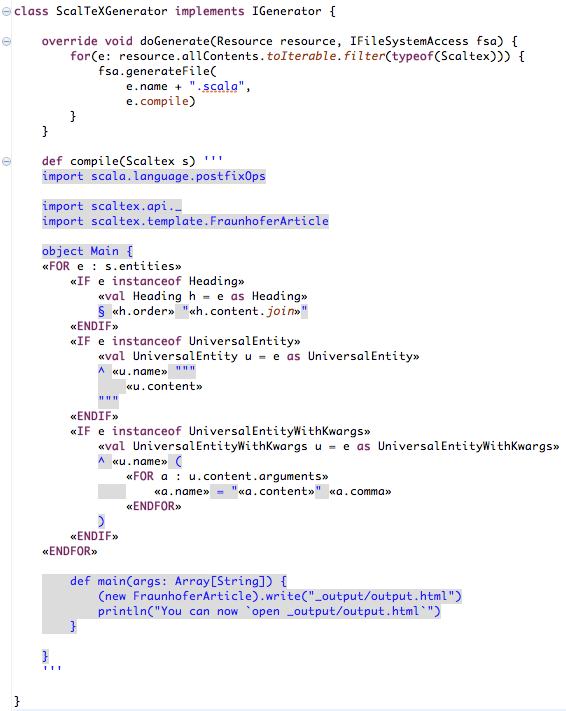
\includegraphics[width=0.9\textwidth]{figures/igenerator.png}
  \caption{IGenerator generiert eine scala-Datei aus der Grammatik von Listing \ref{xtext-gramm}.}\label{fig-igenerator}
\end{figure}

Der ModelInferrer zielt direkt auf die JVM bzw. Java ab und ermöglicht es
u.a. JVM-Datentypen direkt mit in die DSL einzubetten, mit allen Möglichkeiten
die Xbase\footnote{Wobei Xbase selbst mit Xtext gebaut wurde.}
bietet. Es können also dynamisch Java-Klassen generiert werden, wobei innerhalb
der DSL der Fokus auf das Wesentliche gelegt werden kann und nur dort wo es
wirklich nötig ist können General Purpose Expressions zugelassen werden.
Wobei es anzumerken gilt, dass das nicht ganz transparent geschieht,
es muss ein ModelInferrer geschrieben werden, welcher eben die Java-Klassen
dynamisch generiert.
Dies ist also sehr gut, wenn das Ziel auf Java abgebildet werden soll
und gewollt wird dass auf andere Java-Klassen (wie z.B. java.io.File)
aus der DSL heraus benutzt werden können. Kurz: Unterstützung für Expressions.
Die so entstehenden Java-Dateien müssen aber auch noch vom Domain-Benutzer
kompiliert werden.\cite{xtext}

\paragraph{Scala} hingegen hat die Qual der Wahl was das Templating angeht.
Scala selbst bietet in der Standard-Bibliothek schon
eine Reihe an Möglichkeiten an,
z.B. Multiline-Strings oder XML. Jedoch muss sich der Programmierer ersteinmal
eine Architektur überlegen, wie er von den DSL-Klassen auf die Template-Engine
kommt. Weiterhin muss er auch festlegen, wie er das Resultat behandelt,
z.B. wo es gespeichert wird, welche Dateinamen es bekommt etc.
Allerdings hat man für die Automatisierung mehr Werkzeuge in der Hand,
die insbesondere unabhängig von Eclipse sind. So könnte man sich vorstellen
nach dem generieren direkt einen Kompelierungsschritt anzuschließen und
danach das Kompilat auszuführen.

Der große Vorteil einer internen DSL ist jedoch, dass der DSL-Code auch
direkt als Programm laufen kann -- also komplett ohne Umwege, ohne Generierung.
Zudem kann man von der sehr hohen Freiheit und Flexibilität profitieren,
wobei u.U. viel Handarbeit nötig ist.


\section{Auswertung und Ergebnis}

Wie schon in Kapitel \ref{par-ablauf} erwähnt,
  fällt hier die Entscheidung welche der beiden
  DSL-Technologien zur Implementierung des Prototypen ausgewählt wird.

In der Tabelle aus Kapitel \ref{sec-vergleichsmatrix} werden Xtext und
Scala gegenübergestellt und bewertet.
Dabei wird bei jeder Fähigkeit bewertet,
  ob Xtext oder Scala die besseren Argumente liefert,
  jedoch beziehen sich die Bewertungen auf das hier vorliegende Projekt
angepasst sind und sich somit nicht 1:1 auf beliebige Projekte anwenden lassen.
Die Bewertungen bzw. Gewichtungen müssen also ggf. für jedes Projekt und dessen
spezifischen Anforderungen individuell angepasst werden, falls gewünscht.

Weiterhin gilt zu beachten, dass die Bewertungen ihrer Natur nach sowohl
\emph{intuitiv} als auch \emph{objektiv} gewichtet sind, da eben vieles vom
Betracher abhängt und die Fähigkeiten gewisse Überschneidungen haben.
Am Ende steht jedoch ein einigermaßen objektives Maß,
welche Lösung die meisten Vorteile, mit Blick
auf das vorliegende Projekt bietet.

Ich habe mich dazu entschieden eine Skala zwischen \emph{0 und 3} zu verwenden,
wobei 0 schlechte Unterstützung/Möglichkeit/Funktion bzw.
allgemein für das Projekt ungeschickt bedeutet.


\subsection{Auswertungstabelle}\label{sec-auswertungstabelle}

\begin{longtable}{|p{0.5cm}|p{0.8cm}|p{5cm}|c|c|}

  \hline
  Nr. & Kap. & Fähigkeit & Bewertung: Xtext & Bewertung: Scala \\ \hline \hline
  \endfirsthead

  \hline
  Nr. & Kap. & Fähigkeit & Bewertung: Xtext & Bewertung: Scala \\ \hline
  \endhead

  1
  & \ref{sec-grammatikGestaltung}
  & Grammatikalische Gestaltung der DSL
  & 3
  & 1
  \\\hline

  2
  & \ref{sec-gpl}
  & DSL mit General Purpose mischbar
  & 1
  & 3
  \\\hline

  3
  & \ref{sec-strukturierungsfaehigkeit}
  & Strukturierungsfähigkeit des Codes
  & 1
  & 3
  \\\hline

  4
  & \ref{sec-erweiterbar}
  & Erweiterbarkeit durch Domain User/Community (z.B. für eigene Templates)
  & 0
  & 3
  \\\hline

  5
  & \ref{sec-erweiterbar}
  & Erweiterbarkeit durch Entwickler
  & 3
  & 2
  \\\hline

  6
  & \ref{sec-erweiterbar}
  & Wiederverwendbarkeit bzw. Kombination mit Vorhandenem
  & 1
  & 2
  \\\hline

  7
  & \ref{sec-infrastruktur}
  & Sprach-Infrastruktur
  & 3
  & 3
  \\\hline

  8
  & \ref{sec-scalierEinbett}
  & Einbettbarkeit in beliebige Umgebungen
  & 2
  & 3
  \\\hline

  9
  & \ref{sec-generator}
  & Generator: Zielplatform
  & 3
  & 3
  \\\hline

  10
  & \ref{sec-generator}
  & Generator: Template-Engine
  & 3
  & 2
  \\\hline

  11
  &
  & Entwicklungsaufwand (u.a. Zeit, Einarbeitung)
  & 2
  & 2
  \\\hline

  12
  & \ref{sec-erweiterbar}
  & Software-Lebenszyklus und Wartbarkeit
  & 2
  & 2
  \\\hline

  13
  &
  & Tooling (für DSL Gestaltung)
  & 3
  & 0
  \\\hline

  14
  & \ref{sec-scalierEinbett}
  & Skalierbarkeit
  & 1
  & 3
  \\\hline

  15
  &
  & DSL als Library bzw. Bereitstellung
  & 1
  & 3
  \\\hline

\end{longtable}


\subsection{Ergebnis}

Wenn man die Werte aus der Tabelle \ref{sec-auswertungstabelle} zusammenrechnet
kommnt ein Ergebnis zustande, indem sich \textbf{Scala mit 35 zu
29 Punkten in Vergleich mit Xtext} durchsetzt.

Somit ist für \emph{dieses} Projekt Scala besser geeignet.
Und wird als eigentliche Implementierungsbasis für den Prototyp verwendet.

